 % -*- TeX-engine: xetex; eval: (auto-fill-mode 0); eval: (visual-line-mode 1); -*-
% Compile with XeLaTeX

%%%%%%%%%%%%%%%%%%%%%%%
% Option 1: Slides: (comment for handouts)   %
%%%%%%%%%%%%%%%%%%%%%%%

%\documentclass[slidestop,compress,mathserif,12pt,t,professionalfonts,xcolor=table]{beamer}
%
%% solution stuff
%\newcommand{\solnMult}[1]{
%\only<1>{#1}
%\only<2->{\red{\textbf{#1}}}
%}
%\newcommand{\soln}[1]{\textit{#1}}

%%%%%%%%%%%%%%%%%%%%%%%%%%%%%%%
% Option 2: Handouts, without solutions (post before class)    %
%%%%%%%%%%%%%%%%%%%%%%%%%%%%%%%

 \documentclass[11pt,containsverbatim,handout,xcolor=xelatex,dvipsnames,table]{beamer}

 % handout layout
 \usepackage{pgfpages}
 \pgfpagesuselayout{4 on 1}[letterpaper,landscape,border shrink=5mm]

 % solution stuff
 \newcommand{\solnMult}[1]{#1}
 \newcommand{\soln}[1]{}

%%%%%%%%%%%%%%%%%%%%%%%%%%%%%%%%%%%%
% Option 3: Handouts, with solutions (may post after class if need be)    %
%%%%%%%%%%%%%%%%%%%%%%%%%%%%%%%%%%%%

% \documentclass[11pt,containsverbatim,handout,xcolor=xelatex,dvipsnames,table]{beamer}

% % handout layout
% \usepackage{pgfpages}
% \pgfpagesuselayout{4 on 1}[letterpaper,landscape,border shrink=5mm]

% % solution stuff
% \newcommand{\solnMult}[1]{\red{\textbf{#1}}}
% \newcommand{\soln}[1]{\textit{#1}}

%%%%%%%%%%%%%%%%%%%%%%%%%%%%%%%
% Option 4: Notes Only
%%%%%%%%%%%%%%%%%%%%%%%%%%%%%%%

% % See http://tex.stackexchange.com/questions/114219/add-notes-to-latex-beamer
% \documentclass[10pt,containsverbatim,xcolor=xelatex,dvipsnames,table,notes=only]{beamer}

% % handout layout
% \usepackage{pgfpages}
% \pgfpagesuselayout{2 on 1}[letterpaper, landscape, border shrink=5mm]

% % solution stuff
% \newcommand{\solnMult}[1]{#1}
% \newcommand{\soln}[1]{}

%%%%%%%%%%
% Load style file, defaults  %
%%%%%%%%%%

%%%%%%%%%%%%%%%%
% Themes
%%%%%%%%%%%%%%%%

% See http://deic.uab.es/~iblanes/beamer_gallery/ for mor options

% Style theme
\usetheme{Pittsburgh}

% Color theme
\usecolortheme{seahorse}

% Helvetica Neue Light for most text
\usepackage{fontspec}
\setsansfont{Helvetica Neue Light}

%%%%%%%%%%%%%%%%
% Packages
%%%%%%%%%%%%%%%%

\usepackage{geometry}
\usepackage{graphicx}
\usepackage{amssymb}
\usepackage{epstopdf}
\usepackage{amsmath}  	% this permits text in eqnarray among other benefits
\usepackage{url}		% produces hyperlinks
\usepackage[english]{babel}
\usepackage{colortbl}	% allows for color usage in tables
\usepackage{multirow}	% allows for rows that span multiple rows in tables
\usepackage{color}		% this package has a variety of color options
\usepackage{pgf}
\usepackage{calc}
\usepackage{ulem}
\usepackage{multicol}
\usepackage{textcomp}
\usepackage{listings}
\usepackage{changepage}
\usepackage{tikz}
\usetikzlibrary{trees}		% for probability trees
\usepackage{fancyvrb}	% for colored code chunks
\usepackage{nameref}

%%%%%%%%%%%%%%%%
% Remove navigation symbols
%%%%%%%%%%%%%%%%

\beamertemplatenavigationsymbolsempty
\hypersetup{pdfpagemode=UseNone} % don't show bookmarks on initial view

%%%%%%%%%%%%%%%%
% User defined colors
%%%%%%%%%%%%%%%%

% Pantone 2015 Fall colors
% http://iwork3.us/2015/02/18/pantone-2015-fall-fashion-report/
% update each semester or year

\xdefinecolor{custom_blue}{rgb}{0, 0.32, 0.48} % FROM SPRING 2016 COLOR PREVIEW
\xdefinecolor{custom_darkBlue}{rgb}{0.20, 0.20, 0.39} % Reflecting Pond  
\xdefinecolor{custom_orange}{rgb}{0.96, 0.57, 0.42} % Cadmium Orange
\xdefinecolor{custom_green}{rgb}{0, 0.47, 0.52} % Biscay Bay
\xdefinecolor{custom_red}{rgb}{0.58, 0.32, 0.32} % Marsala

\xdefinecolor{custom_lightGray}{rgb}{0.78, 0.80, 0.80} % Glacier Gray
\xdefinecolor{custom_darkGray}{rgb}{0.35, 0.39, 0.43} % Stormy Weather

%%%%%%%%%%%%%%%%
% Template colors
%%%%%%%%%%%%%%%%

\setbeamercolor*{palette primary}{fg=white,bg= custom_blue}
\setbeamercolor*{palette secondary}{fg=black,bg= custom_blue!80!black}
\setbeamercolor*{palette tertiary}{fg=white,bg= custom_blue!80!black!80}
\setbeamercolor*{palette quaternary}{fg=white,bg= custom_blue}

\setbeamercolor{structure}{fg= custom_blue}
\setbeamercolor{frametitle}{bg= custom_blue!90}
\setbeamertemplate{blocks}[shadow=false]
\setbeamersize{text margin left=2em,text margin right=2em}

%%%%%%%%%%%%%%%%
% Styling fonts, bullets, etc.
%%%%%%%%%%%%%%%%

% title slide
\setbeamerfont{title}{size=\large,series=\bfseries}
\setbeamerfont{subtitle}{size=\large,series=\mdseries}
%\setbeamerfont{institute}{size=\large,series=\mdseries}

% color of alerted text
\setbeamercolor{alerted text}{fg=custom_orange}

% styling of itemize bullets
\setbeamercolor{item}{fg=custom_blue}
\setbeamertemplate{itemize item}{{{\small$\blacktriangleright$}}}
\setbeamercolor{subitem}{fg=custom_blue}
\setbeamertemplate{itemize subitem}{{\textendash}}
\setbeamerfont{itemize/enumerate subbody}{size=\footnotesize}
\setbeamerfont{itemize/enumerate subitem}{size=\footnotesize}

% styling of enumerate bullets
\setbeamertemplate{enumerate item}{\insertenumlabel.}
\setbeamerfont{enumerate item}{family={\fontspec{Helvetica Neue}}}
\setbeamerfont{enumerate subitem}{family={\fontspec{Helvetica Neue}}}
\setbeamerfont{enumerate subsubitem}{family={\fontspec{Helvetica Neue}}}

% make frame titles small to make room in the slide
\setbeamerfont{frametitle}{size=\small} 

% set Helvetica Neue font for frame and section titles
\setbeamerfont{frametitle}{family={\fontspec{Helvetica Neue}}}
\setbeamerfont{sectiontitle}{family={\fontspec{Helvetica Neue}}}
\setbeamerfont{section in toc}{family={\fontspec{Helvetica Neue}}}
\setbeamerfont{subsection in toc}{family={\fontspec{Helvetica Neue}}, size=\small}
\setbeamerfont{footline}{family={\fontspec{Helvetica Neue}}}
\setbeamerfont{subsection in toc}{family={\fontspec{Helvetica Neue}}}
\setbeamerfont{block title}{family={\fontspec{Helvetica Neue}}}

%%%%%%%%%%%%%%%%
% New fonts accessed by fontspec package
%%%%%%%%%%%%%%%%

% Monaco font for code
\newfontfamily{\monaco}{Monaco}

%%%%%%%%%%%%%%%%
% Color text commands
%%%%%%%%%%%%%%%%

%orange
\newcommand{\orange}[1]{\textit{\textcolor{custom_orange}{#1}}}

% yellow
\newcommand{\yellow}[1]{\textit{\textcolor{yellow}{#1}}}

% blue
\newcommand{\blue}[1]{\textit{\textcolor{blue}{#1}}}

% green
\newcommand{\green}[1]{\textit{\textcolor{custom_green}{#1}}}

% red
\newcommand{\red}[1]{\textit{\textcolor{custom_red}{#1}}}

% dark gray
\newcommand{\darkgray}[1]{\textit{\textcolor{custom_darkGray}{#1}}}

% light gray
\newcommand{\lightgray}[1]{\textit{\textcolor{custom_lightGray}{#1}}}

% pink
\newcommand{\pink}[1]{\textit{\textcolor{pink}{#1}}}


%%%%%%%%%%%%%%%%
% Custom commands
%%%%%%%%%%%%%%%%

% empty box for probability tree frame
\newcommand{\emptybox}[2]{
	\fbox{ \begin{minipage}{#1} \hfill\vspace{#2} \end{minipage} }
}

% cancel
\newcommand{\cancel}[1]{%
    \tikz[baseline=(tocancel.base)]{
        \node[inner sep=0pt,outer sep=0pt] (tocancel) {#1};
        \draw[red, line width=0.5mm] (tocancel.south west) -- (tocancel.north east);
    }%
}

% degree
\newcommand{\degree}{\ensuremath{^\circ}}

% cite
\newcommand{\ct}[1]{
\vfill
{\tiny #1}}

% Note
\newcommand{\Note}[1]{
\rule{2.5cm}{0.25pt} \\ \textit{\footnotesize{\textcolor{custom_red}{Note:} \textcolor{custom_darkGray}{#1}}}}

% Remember
\newcommand{\Remember}[1]{\textit{\scriptsize{\textcolor{custom_red}{Remember:} #1}}}

% links: webURL, webLink
\newcommand{\webURL}[1]{\urlstyle{same}{\textit{\textcolor{custom_blue}{\url{#1}}}}}
\newcommand{\webLink}[2]{\href{#1}{\textcolor{custom_blue}{{#2}}}}

% mail
\newcommand{\mail}[1]{\href{mailto:#1}{\textit{\textcolor{custom_blue}{#1}}}}

% highlighting: hl, hlGr, mathhl
\newcommand{\hl}[1]{\textit{\textcolor{custom_blue}{#1}}}
\newcommand{\hlGr}[1]{\textit{\textcolor{custom_green}{#1}}}
\newcommand{\mathhl}[1]{\textcolor{custom_blue}{\ensuremath{#1}}}

% example
\newcommand{\ex}[1]{\textcolor{blue}{{{\small (#1)}}}}

% two col: two columns
\newenvironment{twocol}[4]{
\begin{columns}[c]
\column{#1\textwidth}
#3
\column{#2\textwidth}
#4
\end{columns}
}

% slot (for probability calculations)
\newenvironment{slot}[2]{
\begin{array}{c} 
\underline{#1} \\ 
#2
\end{array}
}

% pr: left and right parentheses
\newcommand{\pr}[1]{
\left( #1 \right)
}

%%%%%%%%%%%%%%%%
% Custom blocks
%%%%%%%%%%%%%%%%

% activity: less commonly used
\newcommand{\activity}[2]{
\setbeamertemplate{itemize item}{{{\small\textcolor{custom_orange}{$\blacktriangleright$}}}}
\setbeamercolor{block title}{fg=white, bg=custom_orange}
\setbeamerfont{block title}{size=\small}
\setbeamercolor{block body}{fg=black, bg=custom_orange!20!white!80}
\setbeamerfont{block body}{size=\small}
\begin{block}{Activity: #1}
\setlength\abovedisplayskip{0pt}
#2
\end{block}
}

% app: application exercise
\newcommand{\app}[2]{
\setbeamercolor{block title}{fg=white,bg=custom_green}
\setbeamercolor{block body}{fg=black,bg=custom_green!20!white!80}
\begin{block}{{\small Application exercise: #1}}
#2
\end{block}
}

% disc: discussion question
\newcommand{\disc}[1]{
\vspace*{-2ex}
\setbeamercolor{block body}{bg=custom_blue!25!white!80, fg=custom_blue!55!black!95}
\begin{block}{\vspace*{-3ex}}
#1
\end{block}
\vspace*{-1ex}
}

% clicker: clicker question
\newcommand{\clicker}[1]{
\setbeamercolor{block title}{bg=custom_blue!80!white!50,fg=custom_blue!30!black!90}
\setbeamercolor{block body}{bg=custom_blue!20!white!80,fg=custom_blue!30!black!90}
\begin{block}{\vspace*{-0.2ex}{\footnotesize Clicker question}\vspace*{-0.2ex}}
#1
\end{block}
}

% formula
\newcommand{\formula}[2]{
\setbeamercolor{block title}{bg=custom_blue!40!white!60,fg=custom_blue!55!black!95}
\begin{block}{{\small#1}}
#2
\end{block}
}

% code
\newcommand{\Rcode}[1]{
{\monaco {\footnotesize \textcolor{custom_darkBlue}{#1}}}
}

% output
\newcommand{\Rout}[1]{
{\monaco {\footnotesize \textcolor{custom_darkGray}{#1}}}
}

%%%%%%%%%%%%%%%%
% Change margin
%%%%%%%%%%%%%%%%

\newenvironment{changemargin}[2]{%
\begin{list}{}{%
\setlength{\topsep}{0pt}%
\setlength{\leftmargin}{#1}%
\setlength{\rightmargin}{#2}%
\setlength{\listparindent}{\parindent}%
\setlength{\itemindent}{\parindent}%
\setlength{\parsep}{\parskip}%
}%
\item}{\end{list}}

%%%%%%%%%%%%%%%%
% Footnote
%%%%%%%%%%%%%%%%

\long\def\symbolfootnote[#1]#2{\begingroup%
\def\thefootnote{\fnsymbol{footnote}}\footnote[#1]{#2}\endgroup}

%%%%%%%%%%%%%%%%
% Graphics
%%%%%%%%%%%%%%%%

\DeclareGraphicsRule{.tif}{png}{.png}{`convert #1 `dirname #1`/`basename #1 .tif`.png}

%%%%%%%%%%%%%%%%
% Slide number
%%%%%%%%%%%%%%%%

\setbeamertemplate{footline}{%
    \raisebox{5pt}{\makebox[\paperwidth]{\hfill\makebox[20pt]{\color{gray}
          \scriptsize\insertframenumber}}}\hspace*{5pt}}

          
%%%%%%%%%%%%%%%%
% Remove page numbers
%%%%%%%%%%%%%%%%

\newcommand{\removepagenumbers}{% 
  \setbeamertemplate{footline}{}
}

%%%%%%%%%%%%%%%%
% TOC slides
%%%%%%%%%%%%%%%%

\setbeamertemplate{section in toc}{\inserttocsectionnumber.~\inserttocsection}
\setbeamertemplate{subsection in toc}{$\qquad$\inserttocsubsectionnumber.~\inserttocsubsection \\}

\AtBeginSection[] 
{ 
  \addtocounter{framenumber}{-1} 
  % 
  {\removepagenumbers 
  {\small
    \begin{frame}<beamer> 
    \frametitle{Outline} 
    \tableofcontents[currentsection] 
  \end{frame} 
  } 
  }
} 

\AtBeginSubsection[] 
{ 
  \addtocounter{framenumber}{-1} 
  % 
  {\removepagenumbers 
  {\small
    \begin{frame}<beamer> 
    \frametitle{Outline} 
    \tableofcontents[currentsection,currentsubsection] 
  \end{frame} 
  } 
  }
}
% You cannot use numbers when defining variables.  
% Hence the use of letters, A, B, C, etc.

% Course Name
\newcommand{\CourseName}{Sta 101 - Fall 2015}
\newcommand{\InstituteName}{Duke University, Department of Statistical Science}

% Personal Info
\newcommand{\FirstName}{Mine}
\newcommand{\LastName}{\c{C}etinkaya-Rundel}
\newcommand{\OfficeHours}{Tue + Thur 4:30-6pm}
\newcommand{\OfficeHoursLocation}{Old Chem 213}

% Electronic Info
\newcommand{\PersonalSite}{http://stat.duke.edu/~mc301}
\newcommand{\CourseSite}{http://bit.ly/sta101_f15}
\newcommand{\Email}{mine@stat.duke.edu}

% TAs
\newcommand{\TAA}{Erika Ball}
\newcommand{\TAB}{David Clancy}
\newcommand{\TAC}{Reuben McCreanor}
\newcommand{\TAD}{Anne Driscoll}
\newcommand{\TAE}{Megan Robertson}

% Exam Dates
\newcommand{\ExamADate}{Mon, Oct 5}
\newcommand{\ExamBDate}{Mon, Nov 9}
\newcommand{\FinalDate}{Thur, Dec 10 (2-5pm)}


% ALT ALT
% % You cannot use numbers when defining variables.  
% Hence the use of letters, A, B, C, etc.

% Personal Info
\newcommand{\FirstName}{Anthea}
\newcommand{\LastName}{Monod}
\newcommand{\OfficeHours}{TBA}
\newcommand{\OfficeHoursLocation}{TBA}

% Electronic Info
\newcommand{\PersonalSite}{TBA}
\newcommand{\CourseSite}{TBA}
\newcommand{\Email}{TBA}

% TAs
\newcommand{\TAA}{TBA}
\newcommand{\TAB}{TBA}
\newcommand{\TAC}{TBA}
\newcommand{\TAD}{TBA}
\newcommand{\TAE}{TBA}

% Exam Dates
\newcommand{\ExamADate}{TBA}
\newcommand{\ExamBDate}{TBA}
\newcommand{\FinalDate}{TBA}



%%%%%%%%%%%
% Cover slide info    %
%%%%%%%%%%%

\title{Unit 2: Probability and distributions}
\subtitle{2. Normal distribution}
\author{\CourseName}
\date{}
\institute{\InstituteName}


%%%%%%%%%%%%%%%%%%%%%%%%%
% Begin document and set Helvetica Neue font   %
%%%%%%%%%%%%%%%%%%%%%%%%%

\begin{document}
\fontspec[Ligatures=TeX]{Helvetica Neue Light}

%%%%%%%%%%%%%%%%%%%%%%%%%%%%%%%%%%%

% Title Page

\begin{frame}[plain]

\titlepage

\vfill

{\scriptsize \webLink{\PersonalSite}{Dr. \LastName{}} \hfill Slides posted at  \webURL{\CourseSite}}

\addtocounter{framenumber}{-1} 

\end{frame}

%%%%%%%%%%%%%%%%%%%%%%%%%%%%%%%%%%%%

\section{Housekeeping}

%%%%%%%%%%%%%%%%%%%%%%%%%%%%%%%%%%%%

\begin{frame}
\frametitle{Announcements}

\begin{itemize}

\item Formatting of problem set submissions
\begin{itemize}
\item Bad: Scanned PDF handwriting, unreadable/too dark, haphazard orientation of pages, out
of order
\item Better: Scanned PDF \textbf{neat} handwriting, good scan quality, one file containing
all pages in order
\item Best: Typed using a word processor and PDFed
\end{itemize}

\item Project 1: \webURL{https://stat.duke.edu/courses/Fall15/sta101.002/post/projects/project1.html}
\begin{itemize}
\item Read over before next class and come with questions
\item Start searching for datasets
\item Set team weekly team meetings
\end{itemize}

\end{itemize}

\end{frame}

%%%%%%%%%%%%%%%%%%%%%%%%%%%%%%%%%%%%

\section{Main ideas}

%%%%%%%%%%%%%%%%%%%%%%%%%%%%%%%%%%%%

\subsection{Two types of probability distributions: discrete and continuous}
\label{mi1}

%%%%%%%%%%%%%%%%%%%%%%%%%%%%%%%%%%%%

\begin{frame}
\frametitle{1. Two types of probability distributions: discrete and continuous}

\begin{itemize}

\item A \hl{discrete probability distribution} lists all possible events and the probabilities with 
which they occur
\begin{itemize}
\item The events listed must be disjoint
\item Each probability must be between 0 and 1 
\item The probabilities must total 1
\end{itemize}

\pause

\item A \hl{continuous probability distribution} differs from a discrete probability distribution in 
several ways:
\begin{itemize}
\item The probability that a continuous random variable will equal to any specific value is zero.
\item As such, they cannot be expressed in tabular form.
\item Instead, we use an equation or a formula to describe its distribution via a probability density 
function (pdf).
\item We can calculate the probability for ranges of values the random variable takes (area under 
the curve).
\end{itemize}

\end{itemize}

\end{frame}

%%%%%%%%%%%%%%%%%%%%%%%%%%%%%%%%%%%

\begin{frame}
\frametitle{Examples}

{\small
\twocol{0.6}{0.4}{
\textbf{Discrete:} \\
In a card game if you draw an ace from a well-shuffled full deck you win \$10. If you draw a red card, 
you lose \$2.
\pause
{\footnotesize
\begin{center}
\renewcommand{\arraystretch}{1.5}
\begin{tabular}{l | c | c}
Outcome	(\$)	& X	& P(X) \\
\hline
Win \$10 (black aces)		& 10	& $\frac{2}{52}$ \\
Win \$8 (red aces: 10 - 2)		& 8	& $\frac{2}{52}$ \\
Lose \$2 (non-ace reds)		& -2	& $\frac{24}{52}$ \\
No win / loss	& 0	& $\frac{24}{52}$ \\
\hline
			&	& $\frac{52}{52} = 1$
\end{tabular}
\end{center}
}
}
{
\pause
\textbf{Continuous:} \\
Distribution of female heights is unimodal and nearly symmetric with a mean of 65'' and a standard 
deviation of 3.5'' \webLink{http://www.usablestats.com/lessons/normal}{[source]}.
\vspace{3.3cm}
}
}
\end{frame}

%%%%%%%%%%%%%%%%%%%%%%%%%%%%%%%%%%%%

\subsection{Normal distribution is unimodal, symmetric, and follows the 69-95-99.7 rule}
\label{mi2}

%%%%%%%%%%%%%%%%%%%%%%%%%%%%%%%%%%%%

\begin{frame}
\frametitle{2. Normal distribution is unimodal, symmetric, and follows the 69-95-99.7 rule}

\[ \mathhl{N(\mu,\sigma)} \]

\pause

\begin{itemize}

\item Unimodal and symmetric (bell shaped) that follows very strict guidelines about how variably 
the data are distributed around the mean \\

\pause

\item \hl{68-95-99.7 Rule:}
\begin{itemize}
\item about 68\% of the distribution falls within 1 SD of the mean
\item about 95\% falls within 2 SD of the mean
\item about 99.7\% falls within 3 SD of the mean
\item it is possible for observations to fall 4, 5, or more standard deviations away from the mean, 
but this is very rare if the data are nearly normal
\end{itemize}

\pause

\item Lots of variables are nearly normal, but few are actually normal.

\end{itemize}

\end{frame}

%%%%%%%%%%%%%%%%%%%%%%%%%%%%%%%%%%%

\begin{frame}
\frametitle{}

\clicker{Speeds of cars on a highway are normally distributed with mean 65 miles / hour. The 
minimum speed recorded is 48 miles / hour and the maximum speed recorded is 83 miles / hour. 
Which of the following is most likely to be the standard deviation of the distribution?}

\begin{enumerate}[(a)]
\item -5 \only<2>{\soln{\darkgray{$\rightarrow$ SD cannot be negative}}}
\item \solnMult{5} \only<2>{\soln{\red{$\rightarrow 65 \pm (3 \times 5) = (50, 80)$}}}
\item 10 \only<2>{\soln{\darkgray{$\rightarrow 65 \pm (3 \times 10) = (35, 95)$}}}
\item 15 \only<2>{\soln{\darkgray{$\rightarrow 65 \pm (3 \times 15) = (20, 110)$}}}
\item 30 \only<2>{\soln{\darkgray{$\rightarrow 65 \pm (3 \times 30) = (-25, 155)$}}}
\end{enumerate}

\end{frame}

%%%%%%%%%%%%%%%%%%%%%%%%%%%%%%%%%%%

\subsection{Z scores serve as a ruler for any distribution}
\label{mi3}

%%%%%%%%%%%%%%%%%%%%%%%%%%%%%%%%%%%

\begin{frame}
\frametitle{3. Z scores serve as a ruler for any distribution}

A Z score creates a common scale so you can assess data without worrying about the specific 
units in which it was measured.

\pause

\disc{How can we determine if it would be unusual for an adult woman in North Carolina to be 
96'' (8 ft) tall?}

\pause

\disc{How can we determine if it would be unusual for an adult alien woman(?) to be 103 
metreloots tall, assuming the distribution of heights of adult alien women is approximately normal?}

\end{frame}

%%%%%%%%%%%%%%%%%%%%%%%%%%%%%%%%%%%

\begin{frame}
\frametitle{3. Z scores serve as a ruler for any distribution}

\[ Z = \frac{obs - mean}{SD} \]

\begin{itemize}

\item Z score: number of standard deviations the observation falls above or below the mean

\pause

\item Defined for distributions of any shape, but only when the distribution is normal can we use 
Z scores to calculate percentiles

\pause

\item Observations with $|Z| > 2$ are usually considered \hl{unusual}

\end{itemize}

\end{frame}

%%%%%%%%%%%%%%%%%%%%%%%%%%%%%%%%%%%

\subsection{Z distribution is normal with $\mu = 0$ and $\sigma = 1$}
\label{mi4}

%%%%%%%%%%%%%%%%%%%%%%%%%%%%%%%%%%%%

\begin{frame}
\frametitle{4. Z distribution is normal with $\mu = 0$ and $\sigma = 1$}

\begin{itemize}

\item Linear transformations of a normally distributed random variable will also be normally 
distributed.

\pause

\item Hence, if

\[ Z = \frac{X - \mu}{\sigma}, \text{ where } X \sim N(\mu, \sigma), \]

then

\[ Z \sim N(0,1) \]

\pause

\item Z distribution is a special case of the normal distribution where $\mu = 0$ and $\sigma = 1$ 
(unit normal distribution).

\pause

\item The Z distribution is also called the ``standard normal'' distribution.

\end{itemize}

\end{frame}

%%%%%%%%%%%%%%%%%%%%%%%%%%%%%%%%%%%

\begin{frame}
\frametitle{}

\clicker{Scores on a standardized test are normally distributed with a mean of 100 and a 
standard deviation of 20. If these scores are converted to standard normal Z scores, which of 
the following statements will be correct?}

\begin{enumerate}[(a)]
\item The mean will equal 0, but the median cannot be determined.
\item The mean of the standardized Z-scores will equal 100.
\item The mean of the standardized Z-scores will equal 5.
\item \solnMult{Both the mean and median score will equal 0.}
\item A score of 70 is considered unusually low on this test.
\end{enumerate}

\end{frame}

%%%%%%%%%%%%%%%%%%%%%%%%%%%%%%%%%%%%

\subsection{Normally distributed data plot as a straight line on the normal probability plot}
\label{mi5}

%%%%%%%%%%%%%%%%%%%%%%%%%%%%%%%%%%%%

\begin{frame}
\frametitle{Normal probability plot}

A histogram and \hl{normal probability plot} of a sample of 100 male heights.

\begin{center}
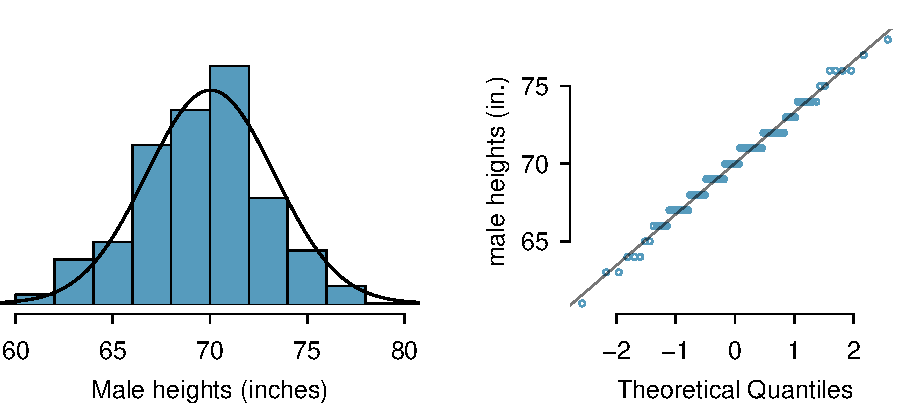
\includegraphics[width=0.9\textwidth]{figures/fcidMHeights/fcidMHeights}
\end{center}

\disc{Why do the points on the normal probability have jumps?}

\end{frame}

%%%%%%%%%%%%%%%%%%%%%%%%%%%%%%%%%%%

\begin{frame}

\disc{Below is a histogram and normal probability plot for the heights of Duke men's basketball 
players (from 1990s and 2000s). Do these data appear to follow a normal distribution?}

\begin{center}
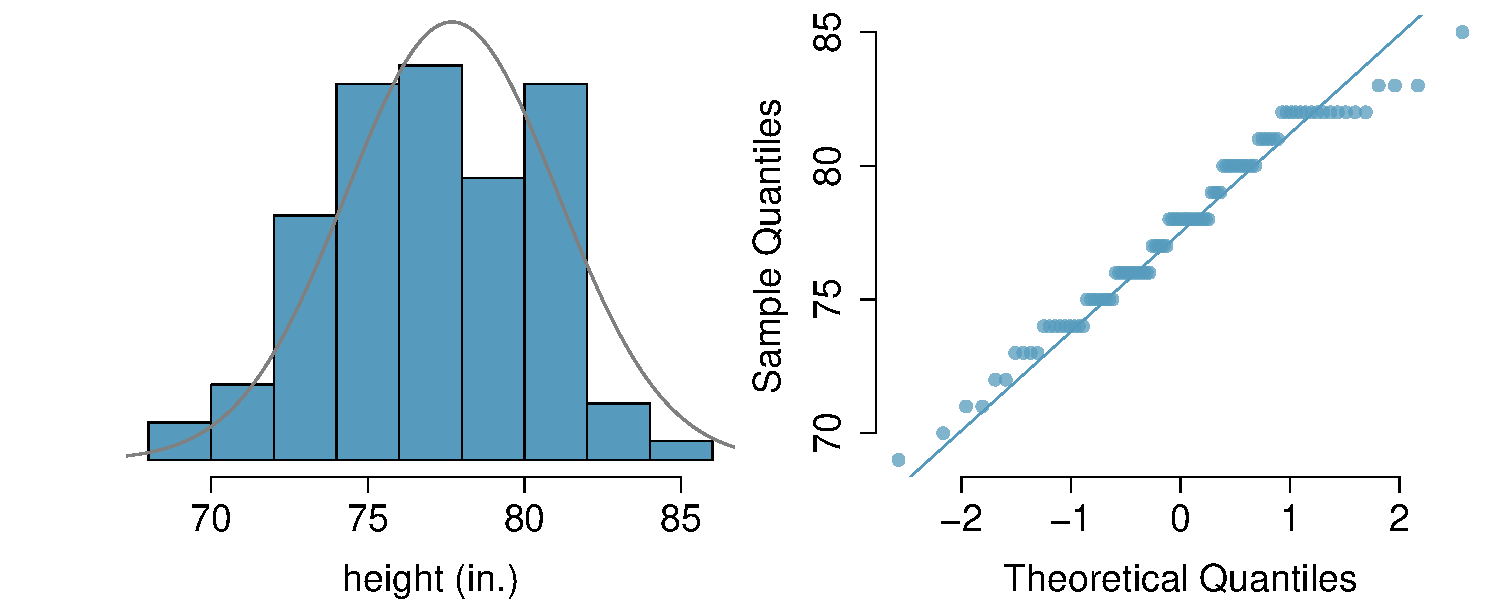
\includegraphics[width=\textwidth]{figures/qq_duke/qq_duke}
\end{center}

\vfill

\ct{Source: GoDuke.com}

\end{frame}

%%%%%%%%%%%%%%%%%%%%%%%%%%%%%%%%%%%

\section{Application exercise}

%%%%%%%%%%%%%%%%%%%%%%%%%%%%%%%%%%%

\begin{frame}
\frametitle{}

\vfill

\app{2.3 Normal distribution}{$\:$\\ See the course website for instructions. \\$\:$}

\vfill

\end{frame}

%%%%%%%%%%%%%%%%%%%%%%%%%%%%%%%%%%%

\section{Summary}

%%%%%%%%%%%%%%%%%%%%%%%%%%%%%%%%%%%

\begin{frame}
\frametitle{Summary of main ideas}

\vfill

\begin{enumerate}

\item \nameref{mi1}

\item \nameref{mi2}

\item \nameref{mi3}

\item \nameref{mi4}

\item \nameref{mi5}

\end{enumerate}

\vfill

\end{frame}

%%%%%%%%%%%%%%%%%%%%%%%%%%%%%%%%%%%

\section{Exercise [time permitting]}

%%%%%%%%%%%%%%%%%%%%%%%%%%%%%%%%%%%

\begin{frame}

\clicker{Which of the following is \underline{false}?}

\begin{enumerate}[(a)]
\item Z scores are helpful for determining how unusual a data point is compared to the rest 
of the data in the distribution.
\item Majority of Z scores in a right skewed distribution are negative.
\item \solnMult{In a normal distribution, Q1 and Q3 are more than one SD away from the mean.}
\item Regardless of the shape of the distribution (symmetric vs. skewed) the Z score of the 
mean is always 0.
\end{enumerate}

\end{frame}

%%%%%%%%%%%%%%%%%%%%%%%%%%%%%%%%%%%

\begin{frame}
\frametitle{}

\disc{{\small At a pharmaceutical factory the amount of the active ingredient which is added 
to each pill is supposed to be 36 mg. The amount of the active ingredient added follows a nearly
normal distribution with a standard deviation of 0.11 mg. Once every 30 minutes a pill
is selected from the production line, and its composition is measured precisely. We know that 
the failure rate of the quality control is 3\% at this factory. What are the bounds of the acceptable 
amount of the active ingredient?}}

\end{frame}

%%%%%%%%%%%%%%%%%%%%%%%%%%%%%%%%%%%

\end{document}